\section{Motor control}
The motor controller should keep the speed of the motor consistent.
In order to ensure this, a P controller is implemented to keep the speed constant of 30 rps.
The motor does not have inbuilt encoders, so in order to get some feedback for the controller, 3 Hall effect sensors are implemented.
A ramp up function is also implemented.

\subsection{Controller}

To ensure a smooth picture the pcb should rotate at a constant speed.
This is done using a P controller, with a gain that is not too big since overshoot is not desirable.

\nikolaj{Maybe a PI controller would be better as we wish to eliminate steady state error.}

\subsection{Encoders} \label{sec:encoders}
%trim = left botm right top
\begin{wrapfigure}{r}{0.7\textwidth}
 \caption{Schematic of the board that is mounted under the spinning board}
 \label{fig:botm_schematic}
 \centering
 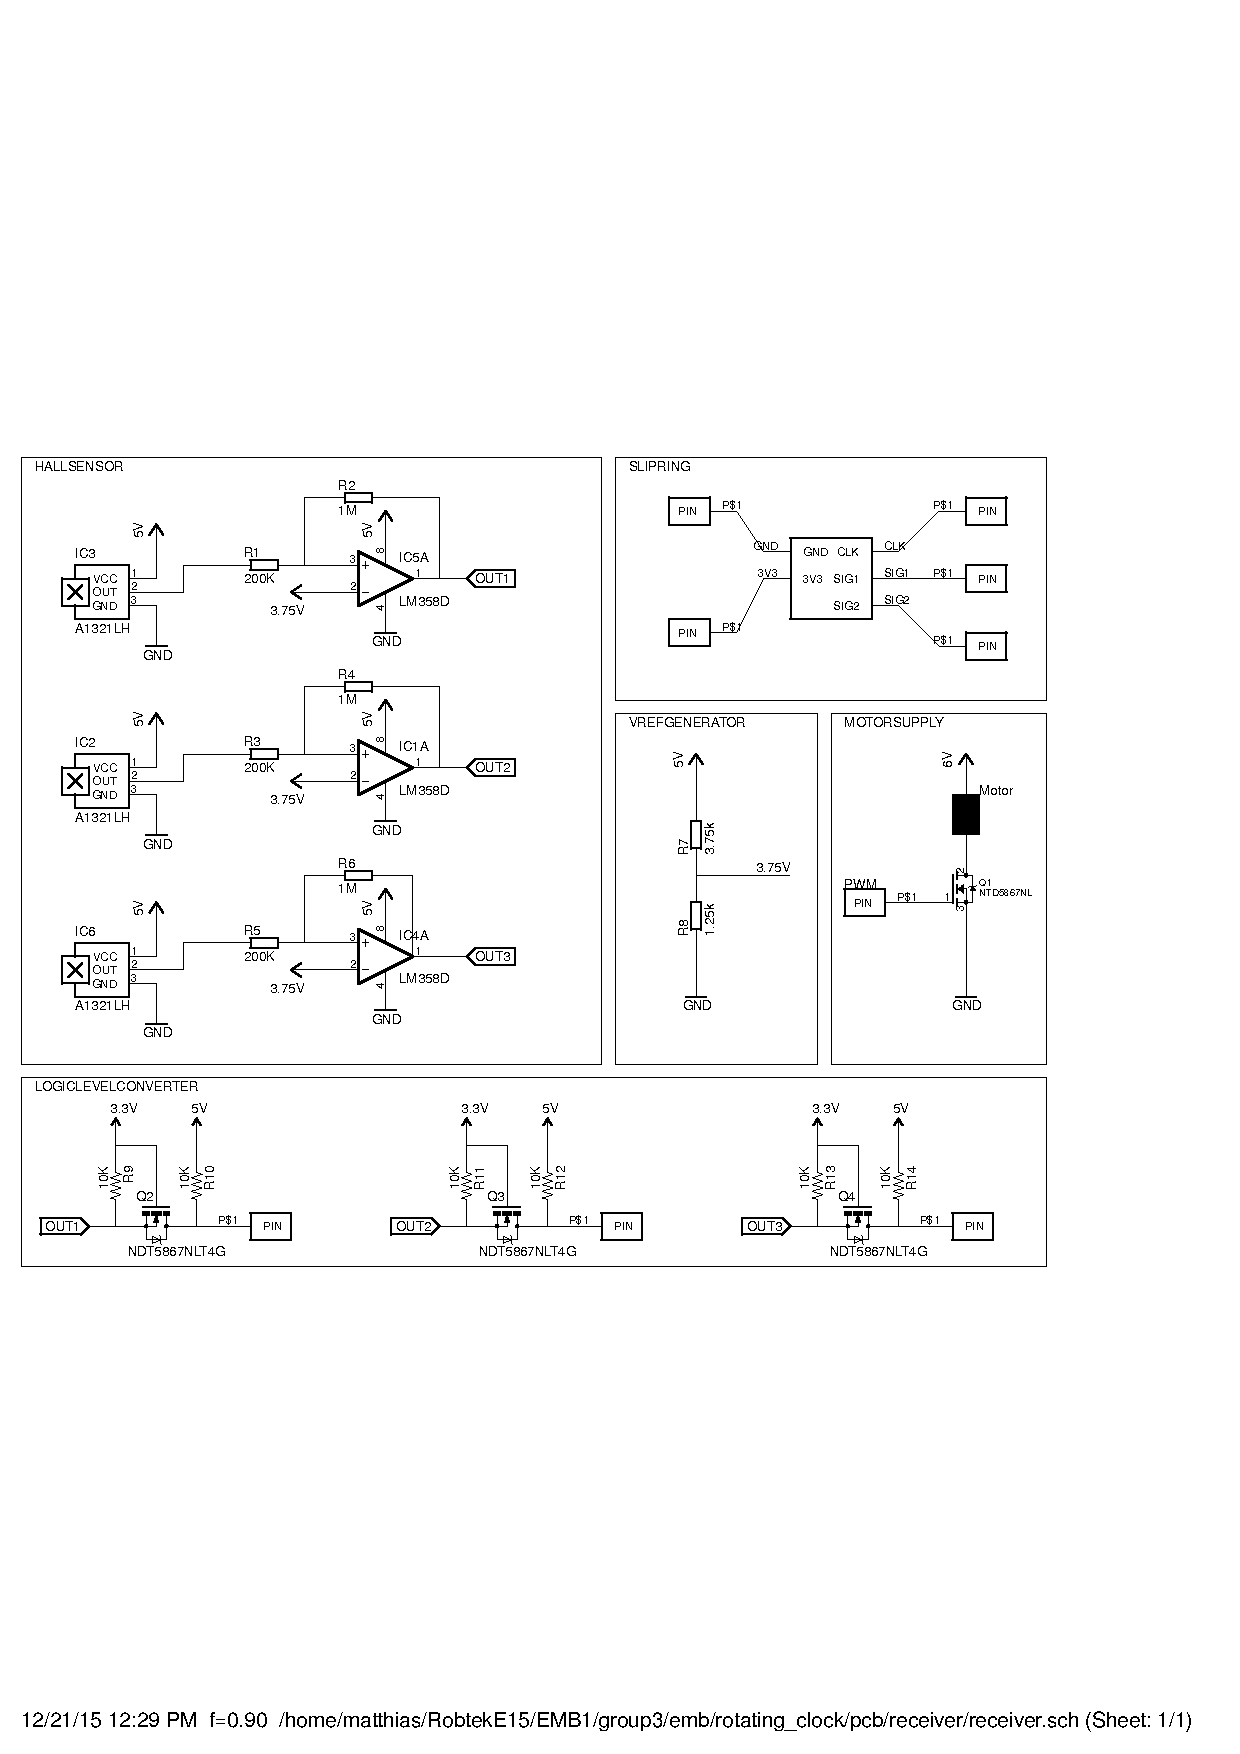
\includegraphics[scale = 0.5,trim = 0 14.5cm 8cm 0,clip = true]{img/bottompcb_schematic}
\end{wrapfigure}

Hall effect sensors responds to magnetic fields.
By mounting a magnet in the rotating board, the Hall sensors will respond when the board is above the sensors, indicating where the board is.
In order to calculate the current speed of the rotating pcb, 3 hall sensor are mounted on the board located under the rotating pcb.
The Hall sensors have been equally distributed with $120^{\circ}$ between them.

In order to get a binary from the analog hall sensor, a Schmitt trigger is added on the output of the hall sensor.
Schmitt trigger is a common amplifier circuit with positive feedback to create hysteresis.
The choice of using a Schmitt trigger instead of a standard comparator is to reduce sensor noise when the magnet is moving over the sensor.
This ensures the signal goes high when the magnet approaches and not going below before the magnet has left.
\nikolaj{We could add a section about how the Schmitt trigger works, with equations and measurements from a breadboard.}

The speed is can be calculated by counting up a counter between getting logic high from one of the hall sensors to  logic high on one of the others, using equations  \ref{eq:calc_time} and \ref{eq:calc_speed}.

\begin{equation} \label{eq:calc_time}
 t = \frac{20\cdot \text{counter}}{1\cdot 10^9}
\end{equation}

\begin{equation} \label{eq:calc_speed}
 \text{speed} = \frac{1}{3\cdot t}
\end{equation}

% \subsubsection{Bottom board}
The schematic for the pcb can be seen in figure \ref{fig:botm_schematic}.

On the board is as mentioned the three hall sensors with a Schmitt trigger for each, as well as the bottom of the slip ring. The slip ring setup and design can be seen in section \ref{sec:ring_connector}. 


\subsection{Ramp up}

The ramp up function is implemented to get a faster speed up time.
If this is not implemented, either an aggressive controller has to be implemented for the entire system, which is not desirable, or the time to reach the desired speed will become very long.

Instead of this, another controller is implemented, which is basically just an integrator.
When the integrator reaches a specified speed, the regular controller takes over. 


\subsection{Driving the motor}

The motor, a normal dc motor, is controlled using pulse width modulation(PWM). The duty cycle is calculated by the controllers as seen in equation \ref{eq:duty}. The maximum speed is defined by the gearing of the motor, and the max RPS at the given voltage, see datasheet \cite{datasheet:motor}. 

\begin{equation}\label{eq:duty}
 \text{duty} = \frac{\text{output}}{\text{max\_speed}}\cdot 100 = \frac{\text{output}}{100\cdot \text{gearing\_ratio}}\cdot 100
\end{equation}

The PWM output is put out on an I/O pin and fed into a transistor capable of sourcing enough current.
A NTD5867NL MOSFET should be able to do this since it can source up to 20 A\cite{datasheet:mosfet}.
